

\chapter{RL Basics}\label{rl_basics}
\setcounter{section}{-1}

\ifx\never_defined\defined
待重读的资源:
\begin{itemize}
%\setlength{\itemsep}{0pt}
%\setlength{\parsep}{0pt}
\setlength{\parskip}{0pt}
\item[-]
\url{https://web.stanford.edu/class/cme241/lecture_slides/david_silver_slides/intro_RL.pdf} \\
\url{../refs/intro_RL.pdf}

\item[-]
\url{https://greentec.github.io/reinforcement-learning-third-en/}

\item[-]
\url{https://yangyangfu.github.io/learning/reinforcement%20learning/2020/05/09/Bellman-Equation/}

\item[-]
\url{https://parkedphoton.com/bellman-equations/}

\item[-]
\url{https://inst.eecs.berkeley.edu/~cs188/sp10/slides/SP10%20cs188%20lecture%2011%20--%20reinforcement%20learning%20(6PP).pdf}

\item[-]
\url{https://www.simplilearn.com/tutorials/artificial-intelligence-tutorial/ai-vs-machine-learning-vs-deep-learning}
\end{itemize}
\fi

Artificial Intelligence is the process of building intelligent machines from vast 
volumes of data. Systems learn from past learning and experiences and perform 
human-like tasks. It enhances the speed, precision, and effectiveness of human 
efforts. AI uses complex algorithms and methods to build machines that can make 
decisions on their own. Machine Learning and Deep learning forms the core of 
Artificial Intelligence. 


%+++++++++++++++++++++++++++++++++++++++++++
\section{Overview}
%-------------------------------------------

Reinforcement learning is useful when you have no training data or specific enough 
expertise about the problem. On a high level, you know WHAT you want, but not really 
HOW to get there. After all, not even Lee Sedol knows how to beat himself in Go.

\begin{figure}[H]
\centering
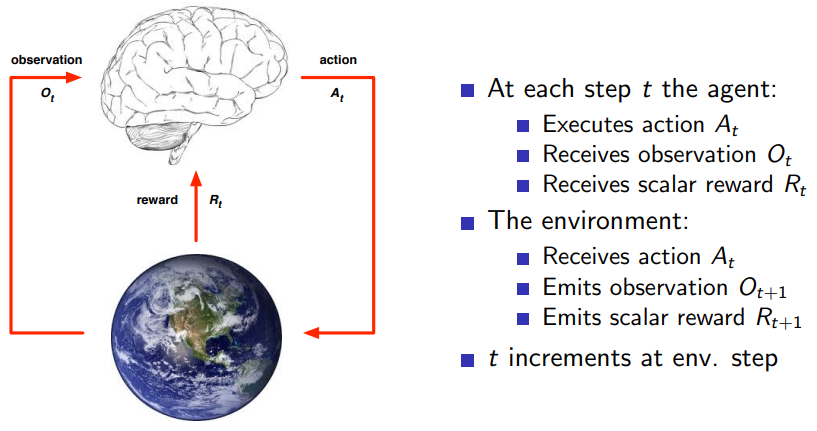
\includegraphics[scale=0.618]{pix/agent_n_env.png}
\caption{Agent and Environment}
%\label{fig:label}
\end{figure}


%+++++++++++++++++++++++++++++++++++++++++++
\subsection{Types of Artificial Intelligence}

The main aim of Artificial Intelligence is to enable machines to perform a human-like 
function. Thus the primary way of classification of AI is based on how well it is able 
to replicate human-like actions. AI can, by and large, be classified based on two 
types, both of which are based on its ability to replicate the human brain. One type 
of classification, which is “Based on Functionality”, classify AI on the basis of their 
likeness to the human mind and their ability to think and feel like humans. The second 
way of classification is more prominent in the tech industry, which is” Based on 
Capabilities” of AI vis-à-vis Human Intelligence.

\begin{figure}[H]
\centering
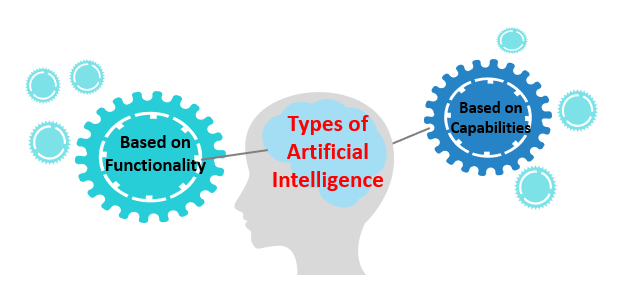
\includegraphics[scale=0.618]{pix/basics/Types-of-AI.png}
\caption{two types of AI which are based on Functionality and Capabilities}
%\label{fig:label}
\end{figure}


\subsubsection{Based on Functionality}

\begin{figure}[H]
\centering
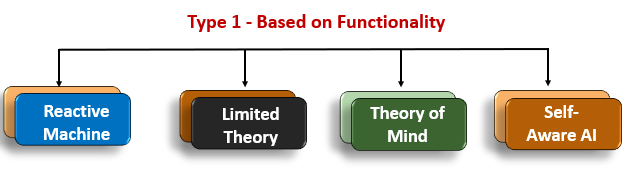
\includegraphics[scale=0.618]{pix/basics/Types-of-Artificial-Intelligence-2.3.png}
\caption{Types based on functionality}
%\label{fig:label}
\end{figure}


\subsubsection{1. Reactive Machine}

They are the most basic and oldest type of Artificial Intelligence. They replicate 
a human's ability to react to different kinds of stimuli. This type of AI has no 
memory power, so they lack the capability to use previously gained 
information/experience to obtain better results. Therefore, these kinds of AI don't 
have the ability to train themselves like the ones we come across nowadays.

{\bf Example:} Deep Blue, IBM's chess-playing supercomputer, is the perfect example 
of these kinds of machines. It is famous for defeating international grandmaster 
Garry Kasparov in the late 1990s. Deep Blue can identify different pieces in the 
chessboard and how each moves. It can identify all the possible legal moves for 
itself and its opponents. Based on the option, it selects the best possible move. 
However, it doesn't have the ability to learn from its past moves as these machines 
don't have any memory of their own.


\subsubsection{2. Limited Theory}

This type of AI, along with the ability of Reactive Machines, have memory capabilities 
so they can use past information/experience to make better future decisions. Most of 
the common applications existing around us fall under this category. These AI 
applications can be trained by a large volume of training data they store in their 
memory in a reference model.

{\bf Example:} Limited Memory technology is used in many self-driving cars use. They 
store data like GPS location, speed of nearby cars, size /nature of obstructions, 
among a hundred other kinds of data to drive just like a human does.


\subsubsection{3. Theory of Mind}

Theory of Mind is the next level of AI, which has very limited to no presence in our 
day-to-day lives. These kind of AI are mostly in the “Work in Progress” stage and are 
usually confined to research labs. These kinds of AI, once developed, will have a very 
deep understating of human minds ranging from their needs, likes, emotions, thought 
process, etc. Basis their understanding of Human minds and their whims, the AI will be 
able to alter its own response.

{\bf Example:} Researcher Winston in his research, showed a prototype of a robot that 
can walk down the small corridor with other robots coming from the opposite direction; 
the AI can foresee other robots movements and can turn right, left or any other way so 
as to avoid a possible collision with the incoming robots. As per Wilson, this Robot 
determines its action based on its “common sense” of how other robots will move.


\subsubsection{4. Self-Aware AI}

This is the final stage of AI. Its current existence is only hypothetical and can be 
found only in Science fiction movies. These kinds of AI can understand and evoke human 
emotions and have emotions of their own. These kind of AI are decades, if not centuries, 
away from materializing. It is this kind of AI which AI skeptics like Elon Musk are 
wary of. This is because once it is self-aware, the AI can get into Self-Preservation 
mode; it might consider humanity as a potential threat and may directly or indirectly 
pursue endeavor to end humanity.


\subsubsection{Based on Capabilities}

\begin{figure}[H]
\centering
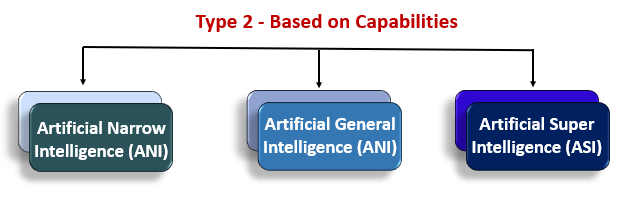
\includegraphics[scale=0.618]{pix/basics/Types-of-Artificial-Intelligence-3.png}
\caption{Types based on capabilities}
%\label{fig:label}
\end{figure}


\subsubsection{1. Artificial Narrow Intelligence (ANI)}

All the existing AI applications which we see around us falls under this category. 
ANI includes an AI system that can perform narrowly defined specific tasks just like 
humans. However these machines cannot perform tasks for which it was not programmed 
before-hand, so they fail at performing an unprecedented task. Based on the 
classification mentioned above, this system is a combination of all reactive and 
limited memory AI. AI algorithms that we use in today's world to perform the most 
complex Prediction Modelling fall under this category of AI.


\subsubsection{2. Artificial General Intelligence (ANI)}

AGI has the capability to train, learn, understand and perform functions just like 
a normal human does. These systems will have multi-functional capabilities cutting 
across different domains. These systems will be more agile and will react and 
improvise just like humans while facing unprecedented scenarios. There is no 
real-world example of this kind of AI, but a good amount of progress has been made 
in this field.


\subsubsection{3. Artificial Super Intelligence (ASI)}

Artificial Super Intelligence will be the top-most point of AI development. ASI 
will be the most potent form of intelligence to ever exist on this planet. It will 
be able to perform all the tasks better than humans because of its inordinately 
superior data processing, memory, and decision-making ability. Some of the 
researchers fear that the advent of ASI will ultimately result in “Technological 
Singularity”. It is a hypothetical situation in which the growth in technology will 
reach an uncontrollable stage, resulting in an unimaginable change in Human 
Civilization.

At present, it is very hard to foresee how our future will look like when a more 
dexterous form of AI materializes. However, with great certainty, we are still a 
long distance apart to reach that stage as we are just in the very nascent stage 
of the development of advanced AI. For the proponents of AI, we can say that we 
are just scratching the surface to unearth the true potential of AI, and for the 
AI skeptics, it is too soon to get chills about Technological Singularity.


%+++++++++++++++++++++++++++++++++++++++++++
\subsection{Learning Models}

In terms of the feedback, AI learning models can be classified based on the interactions 
with the outside environment, users and other external factors. Factoring its 
representation of knowledge, AI learning models can be classified in two main types: 
inductive and deductive.


如果学习时不尝试去理解环境, 这种方法叫做 model-free。所谓 model 就是用模型来表示环境。
反过来,用一个模型来代表环境的方法就是 model-based 方法。 Qlearning, Sarsa, 
Policy Gradients 都是从环境中得到反馈然后从中学习的 model-free 方法。

Learning is the fundamental building blocks of artificial intelligence it helps in 
improving the knowledge of Artificial intelligence programming. AI learning processes 
focused mainly on processing of a collection of input-output pairs for a specific 
function and predicts the outputs for new inputs. The learning models used in AI and 
ML are
\begin{itemize}
%\setlength{\itemsep}{0pt}
%\setlength{\parsep}{0pt}
\setlength{\parskip}{0pt}
\item[-]
Reinforcement Learning

\item[-]
Supervised Learning

\item[-]
Semi-supervised Learning


\item[-]
Unsupervised Learning
\end{itemize}

Deep learning models are broadly classified into supervised and unsupervised 
models:

{\bf Supervised DL models:}
\begin{itemize}
%\setlength{\itemsep}{0pt}
%\setlength{\parsep}{0pt}
\setlength{\parskip}{0pt}
\item[-]
Artificial Neural Networks (ANNs)

\item[-]
Recurrent Neural Networks (RNNs)

\item[-]
Convolutional Neural Networks (CNNs)
\end{itemize}


{\bf Unsupervised DL models:}
\begin{itemize}
%\setlength{\itemsep}{0pt}
%\setlength{\parsep}{0pt}
\setlength{\parskip}{0pt}
\item[-]
Self Organizing Maps (SOMs)

\item[-]
Boltzmann Machines

\item[-]
Autoencoders
\end{itemize}

\section{Value Functions}
% http://www.incompleteideas.net/book/ebook/node34.html

Almost all reinforcement learning algorithms are based on estimating value functions 
-- functions of states (or of state-action pairs) that estimate how good it is for 
the agent to be in a given state (or how good it is to perform a given action in a 
given state). The notion of "how good" here is defined in terms of future rewards 
that can be expected, or, to be precise, in terms of expected return. Of course the 
rewards the agent can expect to receive in the future depend on what actions it will 
take. Accordingly, value functions are defined with respect to particular policies.

Recall that a policy, $\pi$, is a mapping from each state, $s\in\mathcal{S}$, and 
action, $a\in\mathcal{A}(s)$, to the probability $\pi(s,a)$ of taking action $a$ 
when in state $s$. Informally, the value of a state $s$ under a policy $\pi$, denoted 
$V^\pi(s)$, is the expected return when starting in $s$ and following $\pi$ thereafter. 
For MDPs, we can define $V^\pi(s)$ formally as

\begin{equation}\label{rl-policy-state-value}
V^\pi(s) = \mathbb{E}_\pi\{R_t|s_t = s\} = 
\mathbb{E}_\pi\left\{ \sum_{k=0}^\infty\gamma^k r_{t+k+1} | s_t = s \right\},
\end{equation}
where $\mathbb{E}_\pi\{ \}$ denotes the expected value given that the agent follows 
policy $\pi$, and $t$ is any time step. Note that the value of the terminal state, if 
any, is always zero. We call the function $V^\pi$ the {\bf state-value function for 
policy $\pi$}.

Similarly, we define the value of taking action $a$ in state $s$ under a policy $\pi$, 
denoted $Q^\pi(s,a)$, as the expected return starting from $s$, taking the action $a$, 
and thereafter following policy $\pi$:

\begin{equation}\label{rl-policy-action-value}
Q^\pi(s, a) = \mathbb{E}_\pi\{R_t|s_t = s, a_t = a\} = 
\mathbb{E}_\pi\left\{ \sum_{k=0}^\infty\gamma^k r_{t+k+1} | s_t = s, a_t = a \right\},
\end{equation}
We call $Q^\pi$ the {\bf action-value function for policy $\pi$}.

The value functions $V^\pi$ and $Q^\pi$ can be estimated from experience. For example, 
if an agent follows policy $\pi$ and maintains an average, for each state encountered, 
of the actual returns that have followed that state, then the average will converge to 
the state's value, $V^\pi(s)$, as the number of times that state is encountered 
approaches infinity. If separate averages are kept for each action taken in a state, 
then these averages will similarly converge to the action values, $Q^\pi(s,a)$. We call 
estimation methods of this kind Monte Carlo methods because they involve averaging over 
many random samples of actual returns. These kinds of methods are presented in MC methods. 
Of course, if there are very many states, then it may not be practical to keep separate 
averages for each state individually. Instead, the agent would have to maintain $V^\pi$ 
and $Q^\pi$ as parameterized functions and adjust the parameters to better match the 
observed returns. This can also produce accurate estimates, although much depends on 
the nature of the parameterized function approximator.

\begin{emp_box}
需要用到的符号

A Markov Decision Process is a tuple $<\mathcal{S}, \mathcal{A}, \mathcal{P}, 
\mathcal{R}, \gamma>$
\begin{itemize}
%\setlength{\itemsep}{0pt}
%\setlength{\parsep}{0pt}
\setlength{\parskip}{0pt}
\item[-]
$\mathcal{S}$ is a set of states called state space

\item[-]
$\mathcal{A}$ is a set of actions called action space

\item[-]
$\mathcal{P}$ is a state transition probability matrix \\
$\mathcal{P}^a_{ss'}=P(S_{t+1}=s'|S_t=s,A_t=a)$

\item[-]
$\mathcal{R}$ is a reward function \\
$ \mathcal{R}^a_s=\mathbb{E}\left[R_{t+1}|S_t=s,A_t=a\right]$

\item[-]
$\gamma\in[0, 1]$ is a discount factor for future reward
\end{itemize}

\end{emp_box}

A fundamental property of value functions used throughout reinforcement learning and 
dynamic programming is that they satisfy particular recursive relationships. For any 
policy $\pi$ and any state $s$, the following consistency condition holds between the 
value of $s$ and the value of its possible successor states:
\begin{align} 
V^\pi(s)&\doteq \mathbb{E}_\pi \{R_t|s_t=s \} \notag \\
&=\mathbb{E}_\pi\left[\sum_{k=0}^\infty\gamma^k r_{t+k+1}|s_t=s\right] \notag \\
&=\mathbb{E}_\pi\left\{r_{t+1} + \gamma\sum_{k=0}^\infty\gamma^k r_{t+k+2}|s_t=s\right\} \notag \\
&=\sum_{a}\pi(s, a)\sum_{s'}\mathcal{P}_{ss'}^a\left[ \mathcal{R}_{ss'}^a + \gamma
\mathbb{E}_\pi\left\{ \sum_{k=0}^\infty\gamma^k r_{t+k+2}|s_{t+1}=s' \right\} \right] \notag \\
&=\sum_{a}\pi(s,a)\sum_{s'}\mathcal{P}_{ss'}^a\left[ \mathcal{R}_{ss'}^a + 
\gamma V^\pi(s')\right], \label{Bellman_equation_state_value_function_policy}
\end{align}
where it is implicit that the actions, $a$, are taken from the set $\mathcal{A}(s)$, 
and the next states, $s'$, are taken from the set $\mathcal{S}$, or from $\mathcal{S}^*$ 
in the case of an episodic problem. Equation (\ref{Bellman_equation_state_value_function_policy}) 
is the Bellman equation for $V^\pi$. It expresses a relationship between the value of 
a state and the values of its successor states. Think of looking ahead from one state 
to its possible successor states, as suggested by Figure \ref{fig:backup_diagrams_rl}a. 
Each open circle represents a state and each solid circle represents a state-action pair. 
Starting from state $s$, the root node at the top, the agent could take any of some set 
of actions -- three are shown in Figure \ref{fig:backup_diagrams_rl}a. From each of these, 
the environment could respond with one of several next states, $s'$, along with a reward, 
$r$. The Bellman equation (\ref{Bellman_equation_state_value_function_policy}) averages 
over all the possibilities, weighting each by its probability of occurring. It states 
that the value of the start state must equal the (discounted) value of the expected next 
state, plus the reward expected along the way.

\begin{figure}[H]
\centering
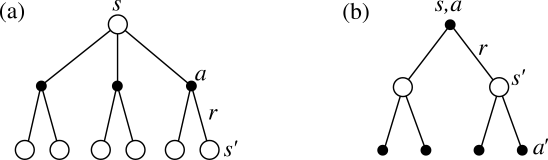
\includegraphics[scale=0.618]{pix/backup_diagrams_rl.png}
\caption{Backup diagrams for (a) $V^\pi$ and (b) $Q^\pi$.}
\label{fig:backup_diagrams_rl}
\end{figure}

The value function $V^\pi$ is the unique solution to its Bellman equation. We show in 
subsequent chapters how this Bellman equation forms the basis of a number of ways to 
compute, approximate, and learn $V^\pi$. We call diagrams like those shown in Figure 
\ref{fig:backup_diagrams_rl} backup diagrams because they diagram relationships that 
form the basis of the update or backup operations that are at the heart of 
reinforcement learning methods. These operations transfer value information back to a 
state (or a state-action pair) from its successor states (or state-action pairs). We 
use backup diagrams throughout the book to provide graphical summaries of the 
algorithms we discuss. (Note that unlike transition graphs, the state nodes of backup 
diagrams do not necessarily represent distinct states; for example, a state might be 
its own successor. We also omit explicit arrowheads because time always flows downward 
in a backup diagram.)


\subsection{Examples}


\subsubsection{Example: Gridworld}

Figure \ref{fig:grid_world}a uses a rectangular grid to illustrate value functions for 
a simple finite MDP. The cells of the grid correspond to the states of the environment. 
At each cell, four actions are possible: \colorbox{yellow}{north}, \colorbox{yellow}{south}, 
\colorbox{yellow}{east}, and \colorbox{yellow}{west}, which 
deterministically cause the agent to move one cell in the respective direction on the 
grid. Actions that would take the agent off the grid(处于边缘的格子移向方框外面的动作) 
leave its location unchanged, but also result in a reward of $-1$. Other actions result 
in a reward of $0$, except those that move the agent out of the special states $A$ and $B$. 
\colorbox{yellow}{From state $A$, all four actions yield a reward of $+10$ and take the 
agent to $A'$.} From state $B$, all actions yield a reward of $+5$ and take the agent to $B'$.

\begin{figure}[H]
\centering
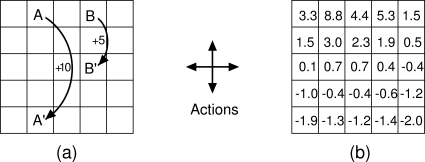
\includegraphics[scale=0.618]{pix/gridworld.png}
\caption{(a) exceptional reward dynamics; (b) state-value function for the equiprobable random policy.}
\label{fig:grid_world}
\end{figure}

\begin{emp_box}
上图中表b是按如下公式计算得出的:
\begin{align} 
V^\pi(s)=\sum_{a}\pi(s,a)\sum_{s'}\mathcal{P}_{ss'}^a\left[ \mathcal{R}_{ss'}^a + 
\gamma V^\pi(s')\right], \tag{\ref{Bellman_equation_state_value_function_policy}}
\end{align}
Recall that the policy $\pi$ is a mapping from each state $s\in\mathcal{S}$ and 
action $a\in\mathcal{A}(s)$ to the probability $\pi(s,a)$ of taking action $a$ 
when in state $s$. The state-value function $V^\pi(s)$ of a state $s$ under a 
policy $\pi$ is the expected return when starting in $s$ and following $\pi$ thereafter.
\end{emp_box}

Suppose the agent selects all four actions with equal probability in all states. Figure 
\ref{fig:grid_world}b shows the value function, $V^\pi$, for this policy, for the 
discounted reward case with $\gamma=0.9$. This value function was computed by solving 
the system of equations (\ref{Bellman_equation_state_value_function_policy}). Notice the 
negative values near the lower edge; these are the result of the high probability of 
hitting the edge of the grid there under the random policy. State A is the best state to 
be in under this policy, but its \textcolor{magenta}{expected return} is less than $10$, its 
\textcolor{magenta}{immediate reward}, 
because from $A$ the agent is taken to $A'$, from which it is likely to run into the edge 
of the grid. State $B$, on the other hand, is valued more than $5$, its immediate reward, 
because from $B$ the agent is taken to $B'$, which has a positive value. From $B'$ the 
expected penalty (negative reward) for possibly running into an edge is more than 
compensated for by the expected gain for possibly stumbling onto $A$ or $B$.


\subsection{Golf}

To formulate playing a hole of golf as a reinforcement learning task, we count a 
penalty (negative reward) of $-1$ for each stroke until we hit the ball into the hole. 
The state is the location of the ball. The value of a state is the negative of the 
number of strokes to the hole from that location. Our actions are how we aim and swing 
at the ball, of course, and which club we select. Let us take the former as given and 
consider just the choice of club, which we assume is either a putter or a driver. The 
upper part of Figure \ref{fig:golf} shows a possible state-value function, $V^{\text{putt}}$, 
for the policy that always uses the putter. The terminal state in-the-hole has a value of 
$0$. From anywhere on the green we assume we can make a putt; these states have value 
$-1$. Off the green we cannot reach the hole by putting, and the value is greater. If 
we can reach the green from a state by putting, then that state must have value one 
less than the green's value, that is, $-2$. For simplicity, let us assume we can putt 
very precisely and deterministically, but with a limited range. This gives us the sharp 
contour line labeled $-2$ in the figure; all locations between that line and the green 
require exactly two strokes to complete the hole. Similarly, any location within putting 
range of the $-2$ contour line must have a value of $-3$, and so on to get all the 
contour lines shown in the figure. Putting doesn't get us out of sand traps, so they 
have a value of $-\infty$. Overall, it takes us six strokes to get from the tee to the 
hole by putting.

\begin{figure}[H]
\centering
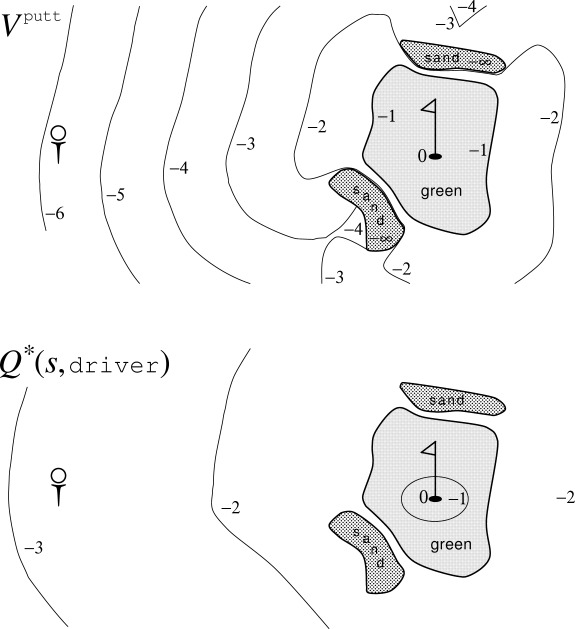
\includegraphics[scale=0.4]{pix/golf.png}
\caption{A golf example: the state-value function for putting (above) and the optimal action-value function for using the driver (below).}
\label{fig:golf}
\end{figure}

